\documentclass{sigchi}

\usepackage{array}
\usepackage{bm}
%\usepackage{longtable}
\usepackage{afterpage}

\usepackage{tabularx}
\newcolumntype{P}[1]{>{\centering\arraybackslash\small}p{#1}}
\newcolumntype{M}[1]{>{\begin{varwidth}[t]{#1}}l<{\end{varwidth}}}
% Use this command to override the default ACM copyright statement
% (e.g. for preprints).  Consult the conference website for the
% camera-ready copyright statement.

 %------------begin Float Adjustment
%%two column float page must be 90% full
%\renewcommand\dblfloatpagefraction{.10}
%%two column top float can cover up to 80% of page
% %renewcommand\dbltopfraction{.80}
%%float page must be 90% full
%\renewcommand\floatpagefraction{.10}
%%top float can cover up to 80% of page
%\renewcommand\topfraction{1}
%%bottom float can cover up to 80% of page
%\renewcommand\bottomfraction{1}
%%at least 10% of a normal page must contain text
%\renewcommand\textfraction{0}
%%separation between floats and text
%\setlength\dbltextfloatsep{9pt plus 5pt minus 3pt }
%%separation between two column floats and text
%\setlength\textfloatsep{4pt plus 2pt minus 1.5pt}

%% EXAMPLE BEGIN -- HOW TO OVERRIDE THE DEFAULT COPYRIGHT STRIP -- (July 22, 2013 - Paul Baumann)
% \toappear{Permission to make digital or hard copies of all or part of this work for personal or classroom use is      granted without fee provided that copies are not made or distributed for profit or commercial advantage and that copies bear this notice and the full citation on the first page. Copyrights for components of this work owned by others than ACM must be honored. Abstracting with credit is permitted. To copy otherwise, or republish, to post on servers or to redistribute to lists, requires prior specific permission and/or a fee. Request permissions from permissions@acm.org. \\
% {\emph{CHI'14}}, April 26--May 1, 2014, Toronto, Canada. \\
% Copyright \copyright~2014 ACM ISBN/14/04...\$15.00. \\
% DOI string from ACM form confirmation}
%% EXAMPLE END -- HOW TO OVERRIDE THE DEFAULT COPYRIGHT STRIP -- (July 22, 2013 - Paul Baumann)


% Arabic page numbers for submission.  Remove this line to eliminate
% page numbers for the camera ready copy 

%\pagenumbering{arabic}
% \usepackage{booktabs}
% \usepackage[normalem]{ulem}
% \useunder{\uline}{\ul}{}


% Load basic packages
\usepackage{balance}  % to better equalize the last page
\usepackage{graphics} % for EPS, load graphicx instead 
%\usepackage[T1]{fontenc}
\usepackage{txfonts}
\usepackage{times}    % comment if you want LaTeX's default font
\usepackage[pdftex]{hyperref}
% \usepackage{url}      % llt: nicely formatted URLs
\usepackage{color}
\usepackage{textcomp}
\usepackage{booktabs}
\usepackage{ccicons}
\usepackage{todonotes}
\usepackage{multirow}
\usepackage{float}

% llt: Define a global style for URLs, rather that the default one
\makeatletter
\def\url@leostyle{%
  \@ifundefined{selectfont}{\def\UrlFont{\sf}}{\def\UrlFont{\small\bf\ttfamily}}}
\makeatother
\urlstyle{leo}

% To make various LaTeX processors do the right thing with page size.
\def\pprw{8.5in}
\def\pprh{11in}
\special{papersize=\pprw,\pprh}
\setlength{\paperwidth}{\pprw}
\setlength{\paperheight}{\pprh}
\setlength{\pdfpagewidth}{\pprw}
\setlength{\pdfpageheight}{\pprh}

% Make sure hyperref comes last of your loaded packages, to give it a
% fighting chance of not being over-written, since its job is to
% redefine many LaTeX commands.
\definecolor{linkColor}{RGB}{6,125,233}
\hypersetup{%
  pdftitle={SIGCHI Conference Proceedings Format},
  pdfauthor={LaTeX},
  pdfkeywords={SIGCHI, proceedings, archival format},
  bookmarksnumbered,
  pdfstartview={FitH},
  colorlinks,
  citecolor=black,
  filecolor=black,
  linkcolor=black,
  urlcolor=linkColor,
  breaklinks=true,
}

%shortcut for comments
\newcommand{\comment}[1]{\textcolor{red}{#1}}
\newcommand{\boldit}[1]{\textbf{\textit{#1}}}

% create a shortcut to typeset table headings
% \newcommand\tabhead[1]{\small\textbf{#1}}

% End of preamble. Here it comes the document.
\begin{document}

\title{Spin-lock Gesture Authentication for Android: Usability in a Soft-Interface}

\numberofauthors{4}
\author{%
  \alignauthor{Stefania Raimondo\\
    \affaddr{University of Toronto}\\
    \affaddr{Toronto, Canada}\\
    \email{stefania.raimondo@mail.utoronto.ca}}\\
  \alignauthor{Alan Yusheng Wu\\
    \affaddr{University of Toronto}\\
    \affaddr{Toronto, Canada}\\
    \email{yusheng.wu@mail.utoronto.ca}}\\
  \alignauthor{Yomna Aly\\
    \affaddr{University of Toronto}\\
    \affaddr{Toronto, Canada}\\
    \email{yomna.aly@mail.utoronto.ca}}\\
  \alignauthor{Molly Wei\\
    \affaddr{University of Toronto}\\
    \affaddr{Toronto, Canada}\\
    \email{molly.wei@mail.utoronto.ca}}\\
}

\maketitle

\begin{abstract}
The screen-lock mechanisms currently distributed with touch-screen mobile devices suffer from usability issues that hinder their adoption and from security risks such as observatory and smudge attacks. We have developed an alternative touch-based authentication method, based on the single dial combination lock, with the goal of providing improved protection to users. We performed a between participant study, with 21 young adult participants, to compare the usability of this new interface to that of the prevalent Pin and Pattern Android locks. 63 successful unlocking trials were conducted on each interface using a range of easy, medium and hard passwords. The Pattern lock had the fastest unlock time, while the new Spin lock had the slowest. However, users 
\comment{TODO}
 Significant differences were found between the three locks in terms of unlock speed, error rate, and User Acceptance. Ultimately, the pattern lock proved to be significantly faster and less error prone than the other two. Nonetheless, the spin lock was accepted and enjoyed by users despite their unfamiliarity with the new interface.

\end{abstract}

\keywords{lockscreens; lock; authentication; smart phone; combination lock}

\iffalse
\category{H.5.m.}{Information Interfaces and Presentation
  (e.g. HCI)}{Miscellaneous} \category{See
  \url{http://acm.org/about/class/1998/} for the full list of ACM
  classifiers. This section is required.}{}{}
\fi


\section{Introduction}
Mobile devices contain an immense amount of confidential information and provide access to personal services such as banking, emailing, and social networking. Yet over 50\% of smartphone users disable the lock-screen authentication mechanisms provided by manufacturers~\cite{consumer_reports_smart_2014} due to the inconvenience associated with repeated unlocking~\cite{egelman_are_2014}. For lock-screen users, the amount of time spent unlocking can accumulate to up to one hour per month, and less than one quarter of these unlocks are considered necessary by the user~\cite{riva_progressive_2012,harbach_itsa_2014}. 

Currently, popular touch-screen authentication methods include the text-based password, the PIN lock where users enter a sequence of digits, and the gesture-based pattern lock that requires users to swipe specific patterns through a 3x3 grid of dots on the screen~\cite{andriotis_pilot_2013}. However, all of these lock interfaces suffer from usability issues that result in security risks even if they are adopted by users. For example, although text-based passwords provide a large space of complex passwords, these are time-consuming to input, are error-prone, and are difficult for users to memorize~\cite{schloglhofer_secure_2012,andriotis_pilot_2013,egelman_are_2014}. Thus, users opt to use predictable passwords, reuse passwords, or abandon them~\cite{biddle_graphical_2012} entirely. Unfortunately, PIN and pattern locks also suffer from predictable password selection~\cite{uellenbeck_quantifying_2013,arif_use_2014,arif_tap_2013}, and these have significantly smaller input spaces than text-based passwords. 

Another security risk associated with all of the mentioned methods, and especially the pattern lock, comes from observational attacks. These include Shoulder Surfing~\cite{von_zezschwitz_making_2013,egelman_are_2014}, where an attacker directly observes password entry in a public setting, and Smudge Attacks, where an attacker infers a password based solely on the oily residues or ``smudges" left on the device~\cite{egelman_are_2014}. Much research has been aimed at reducing these risks: ~\cite{arif_use_2014} incorporates pressure input and ~\cite{arif_tap_2013} incorporates swiping gestures into PINs, while ~\cite{schneegass_smudgesafe:_2014,von_zezschwitz_making_2013} allows patterns to be inputted on unique images that may be transformed via rotation and shape alteration. However, the former reduces input speed and password usability, on top of requiring extra hardware ~\cite{arif_use_2014,arif_tap_2013}, while the latter still suffers from predictable password selection based on landmarks in the images ~\cite{andriotis_pilot_2013}.

Other active screen-lock research has moved away from touch interfaces and towards using external devices~\cite{winkler_glass_2015}, biometrics~\cite{clarke_advanced_2007}, implicit context~\cite{micallef_why_2015,schloglhofer_secure_2012,von_zezschwitz_patterns_2013} or machine learning~\cite{riva_progressive_2012}. Although these designs show promising results, they are still relatively immature and unreliable~\cite{schneegass_smudgesafe:_2014}. In some cases, they actually reduce security in favor of usability~\cite{khan_itus:_2014, micallef_why_2015}. Furthermore,  ~\cite{riva_progressive_2012} suggests that there remains a need for explicit authentication in certain circumstances.

In this study, we propose an alternative touch-based explicit authentication method for mobile devices based on the single dial combination lock. This is inspired partially by users' affinity to the swipe-based pattern lock for its ease of use ~\cite{van_bruggen_modifying_2013}, despite having slower input speeds and higher error rates than PIN passwords~\cite{von_zezschwitz_patterns_2013}. It is also inspired by the ubiquity and ease-of-use of the physical combination lock as well as the potential for reducing informative ``smudge" residues with overlapping circular gestures. To our knowledge, no research has been performed into the usability or security of a spin-lock based lock-screen, or the transferability of this mechanism from a physical to soft-interface. As users tend to value efficiency and satisfaction over the security provided by a lock screen~\cite{micallef_why_2015}, our goal is to explore potential improvements in usability which may lead to greater user adoption and, subsequently, better protection for the users. In order to do so, we will investigate the usability of the new spin lock interface and compare it to the existing PIN and pattern interfaces.

\section{Research Question and Hypothesis}
To investigate the usability of our proposed spin-dial combination lock (which we will call the spin lock from this point forward), we will compare it to the PIN and pattern locks with respect to unlock speed, error rate, and user acceptance. Our hypotheses are as follows:

\begin{itemize}
	\item H1: The spin lock and pattern lock will have similar unlock times that are significantly higher than the PIN lock, given same password complexity, due to their similarity in using gesture-based interactions.
	\item H2: The spin lock and pattern lock will have similar error rates that are significantly higher than the PIN lock, given same password complexity, due to their similarity in using gesture-based interactions.
   	\item H3: The spin lock will be received positively by users. However, the PIN and pattern locks will have similar levels of user acceptance and will still be higher than the spin lock due to users' potential familiarity with these existing methods.
\end{itemize}

We predict that the pattern and spin lock will be very similar with regards to speed, error rate and acceptance since they require similar gesture-based interactions to unlock the phone. However, they will be prominently superseded by the PIN lock. We hope that our users report higher user acceptance ratings to the new spin lock interface despite its unfamiliarity.

\section{Methodology}
\subsection {Apparatus}
\subsubsection{Hardware}
A Nexus 5 (2013) running Android 6.0 Marshmallow served as the primary testing platform. This particular model was chosen based on hardware availability and performance characteristics required to create smooth interactions for this study. This device has a 5-inch screen (4.95 inch). \\

\subsubsection{Software Interface}
The software locking mechanisms were implemented as part of an Android application which guides the participant through all stages of the in-lab experiment. The application simulates lock screens onto which a user must correctly enter passwords. While the user interacts with the lock screen, usage statistics were collected in the background by the application for later analysis. 

Three different lock screens were assessed in this study: the pattern lock was developed using a library of the native Android pattern lock, the PIN lock was developed to emulate the functionality of the Android PIN lock, and the Spin lock was developed from scratch with a custom display and custom gestural interactions. The password input method of each lock screen are briefly summarized in Table \ref{tab:interactions}.

\begin{table}[h]
\centering
  \begin{tabular}{c l}
    \toprule
    \small\textit{ Interface} &
    \multicolumn{1}{c}{\small\textit{Unlock Interaction}}\\
    \midrule
    \small\textbf{Pin} & Enter the numeric password using the number pad \\
    \midrule
    \small\textbf{Pattern} & \begin{tabular}{@{}l@{}}Swipe through a pattern of dots    in the 3 x 3 grid \end{tabular}\\
    \midrule
    \small\textbf{Spin} & \begin{tabular}{@{}l@{}} Enter the numeric password by swiping in a circular\\ gesture through the numbers to the target number, \\ changing  the direction of rotation for each digit\\
    \end{tabular}\\ 
    \bottomrule
  \end{tabular}
  \caption{Lock screen interface interaction guidelines}~\label{tab:interactions}
\end{table}

\subsection{Participants}

\begin{figure*}
  \centering
  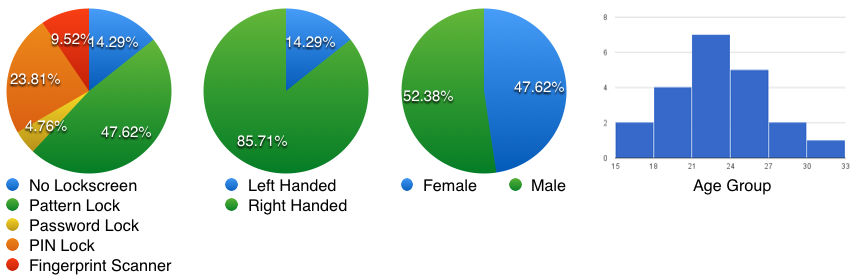
\includegraphics[width=1.6\columnwidth]{figures/user_group_demo}
  \caption{Participants demographics}~\label{fig:usergroup}
\end{figure*}

For this study, 21 lock-screen users were recruited as participants. While this experiment was performed on an Android device, both Android and iPhone users with a variety of lock screen preferences were included to increase the universality of this study. A breakdown of the user demographics are shown in Figure~\ref{fig:usergroup}. No restrictions were placed on user demographics, including physical characteristics, since we expect the effect of these variables on the experiment to be insignificant and thus for the results to generalize well to the population of smart phone users at large.

\subsection{Experimental design}

We performed a controlled within-participant experiment, in which the primary independent variable was the lock screen interface (with three levels: PIN, pattern and spin locks). In order to determine the \textit{general usability} of the interfaces, passwords of varying difficulty were tested. For each interface, 7 passwords of ''easy", ''medium" and ''hard" difficulties were tested by each participant, for a total of 21 passwords per interface. Each password was completed 3 times, for a total of 21 $\times$ 3 = 63 successful trials per interface. 

Password difficulty was measured based on total finger movement, considering both the number of strokes and total distance moved as shown in Table \ref{tab:tablePassword}. Participants  tested all passwords in each difficulty level in a random order, but tested the password levels in order of increasing difficulty. Given that ``identical'' passwords cannot be used across interfaces, even with careful password selection, the password remains a confounding variable. Furthermore, passwords were selected in order to provide a representative measure of the overall usability of the interface and do not necessarily conform to users' "real-life" password selection. 

\begin{table}[h]
\centering
  \begin{tabular}{c c c}
    \toprule
    \small \textit{Complexity} & 
    \small \textit{No. of Strokes} & 
    \small \textit{Distance}\\
    \midrule
    \small \textbf{Easy} & 2$\sim$3 & 7.5$\sim$8 cm \\
    \midrule
    \small \textbf{Medium} & 3$\sim$4 & 10$\sim$10.5 cm \\
    \midrule
    \small \textbf{Hard} & 4$\sim$5 & 15$\sim$15.5 cm \\
    \bottomrule
  \end{tabular}
  \caption{Password complexity specifications}~\label{tab:tablePassword}
\end{table}

Additionally, the order in which the interfaces were tested was counterbalanced across participants using Latin squares to compensate for order effects.To compensate for potential fatigue, participants were also given 30 seconds break every 21 trials (or between each difficulty level). Lastly, in an attempt to compensate for learning effects from both the interfaces and the testing platform, participants were given a tutorial for each interface and a 5-minute period to practice unlocking with a distinct set of practice passwords. 

The controlled trials in this experiment were run with identical setup, ambiance and testing procedure. Participants were also asked to perform tasks with their dominant hand only in order to reduce variance caused by input preferences.

\subsection{Tasks and procedures}
\textit{Step 1, Introduction: }
Participants were introduced to the study and given an overview of the tasks in the experiment. Emphasis was placed on performing the tasks to the best of their ability and as quickly as possible. They were also told that they must utilize their dominant hand only when unlocking the interfaces. Participants were then presented with the test phone with the test application pre-loaded , ready to start the experiment.

\textit{Step 2, Interface Demo Video: }
Participants were introduced to each interface through a demonstration video played by the test application explaining how to unlock the interface. 

\textit{Step 3, Interface Practice Time: }
Participants were given up to 5 minutes to practice using the lock screen before trials began. The practice session interface was identical to test interface except that the practice passwords were a distinct set from those used in the test. 
 
\textit{Step 4, Interface Trials: } 
Each participant performed the unlocking task using passwords presented by the application on the lock screen. If the participant incorrectly entered a password, the application notified them of the failed attempt and asked them to enter it again. Only a successful password entry constituted a completed trial. The test interfaces are shown in Figure~\ref{fig:test_interfaces}.

\begin{figure}[h]
  \centering
  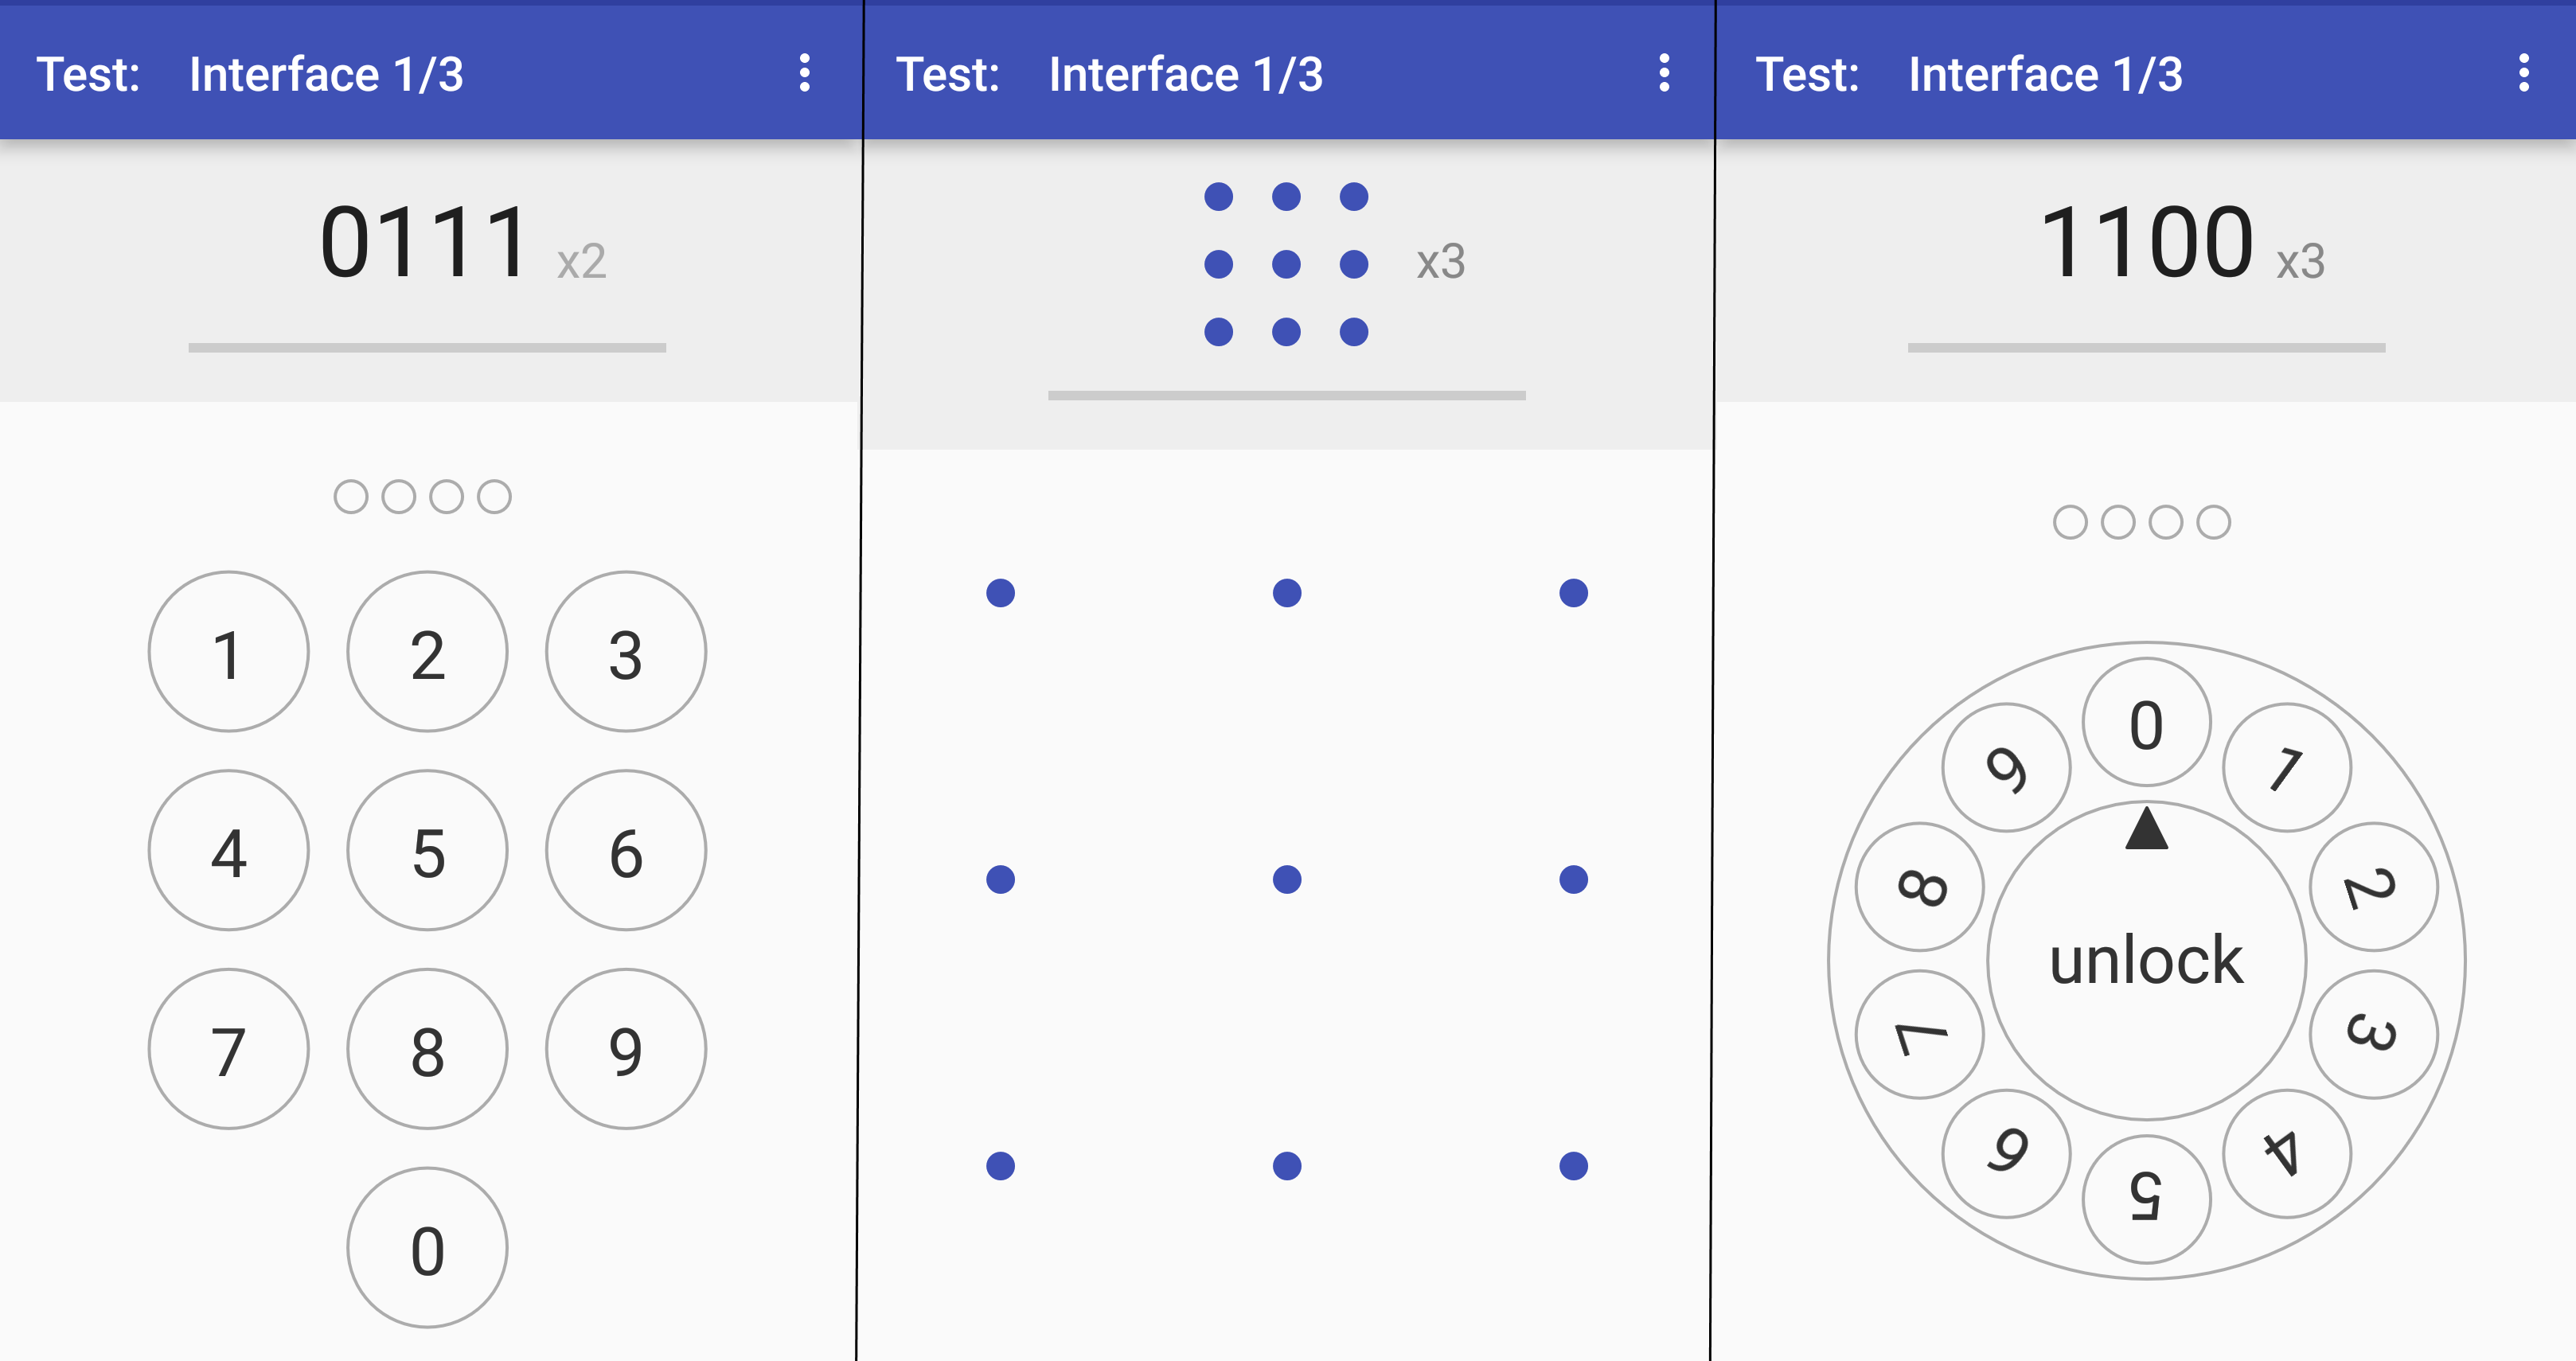
\includegraphics[width=1\columnwidth]{figures/screenshot_test_all.png}
  \caption{Test interfaces, from left to right: PIN, Pattern, SPIN}~\label{fig:test_interfaces}
\end{figure}

After completing each difficulty level of passwords on a given interface, the participants were given a 30 second break. 

\textit{Step 5, Repeat: }
Steps 2-4 were repeated for the subsequent two interfaces.

\textit{Step 6, Post-experiment: }
After the participants had completed the experiment, they filled out the Post Study Questionnaire about their experience with the various interfaces. The survey collected the users' subjective evaluation of the usability of the interfaces and users' willingness to adopt them on their personal devices. Additional comments were also collected.

\subsection{Measures}
The following dependent variables measured during this experiment were selected in order to evaluate the usability of the three locking interfaces:

\textit{1) Unlock Speed: }
Unlock speed (equivalently, password entry time) was measured for each trial and compared across interfaces. Entry time was only measured for successful password entries; unsuccessful trials were accounted for through error rate calculations. The unlock speed was measured from the moment that the participant touched the screen to begin password entry to the moment that a successful password entry had been completed. 

\textit{2) Error Rate: }
Error rate is measured as the ratio of the number of failed attempts to the total number of attempts. Each password entry attempt was identified as either a success or failure. Thus, while a given password is used for three trials, it may be entered in more than three password attempts. Per trial error rate is taken as the percentage of failed attempts per trial. 

\textit{3) Acceptance/Perception: }
Error rate and unlock speed, as demonstrated by users' preference of the pattern lock over the PIN~\cite{van_bruggen_modifying_2013, von_zezschwitz_patterns_2013}, are not sufficient to determine whether an interface is deemed highly ``usable'' and preferred by users, thus we uses qualitative measures to ascertain user acceptance. To measure user acceptance, participants answered questions regarding perceptions of speed, ease of use,  likelihood of adoption, and feedback of the interfaces. These questions were formatted using the 7-point scale NASA-TLX format. Users were also asked to reflect on difficulties they encountered during the experiment and record their reflections in a free-form manner. During the experimental trials, the experimenter also noted any interesting behavior or comments of the participants. 

\iffalse
\begin{table}[h]
\centering
  \begin{tabular*}{\columnwidth*7/8}{@{}P{\columnwidth*7/8}}
    \toprule
    \small\textit{ Question} \\
    \midrule
    Would you adopt this locking mechanism on your own phone? \\ 
    \midrule
    How easy did you find using this lock mechanism? \\
    \midrule
    Was feedback clear regarding whether or not a password attempt was a success or a failure? \\
    \midrule 
    How quickly did you feel you were able to enter your password with this interface? \\
    \midrule
    Was it easy to input your password correctly and accurately? \\
    \midrule
    Please Specify any kind of difficulty encountered when using the lock mechanism? \\ 
    \bottomrule
  \end{tabular*}
  \caption{Post-experiment survey questions}~\label{tab:survey_questions}
\end{table}
\fi

\subsection {Data collection }
Data were collected through two methods: quantitative data on unlock speed and error rate was collected by the testing application, and qualitative data on user's subjective opinion was collected using questionnaires. 

\section{Results}

\subsection{Unlock Speed}
Average unlock times of successful attempts for each interface are provided in Figure ~\ref{fig:unlock_speed_bar}. Significant differences were observed between unlock times (Anova: $F_2=186.64$, $p < 0.001$), with a Tukey-Kramer post-hoc test indicating that the pattern lock was significantly faster than the spin and Pin locks ($p(Pin, Pattern) < 0.001 $, $p(Spin,Pattern)< 0.001$), but no significant difference was observed between the spin and pin locks (with $p > 0.1$).
%UPDATE analysis_1_interface_speed_anova.jpg
 %UPDATE  analysis_1_interface_speed_means.txt 
%UPDATE: analysis_1_interface_speed_anova_posthoc.txt

\begin{figure}[h]
  \centering
  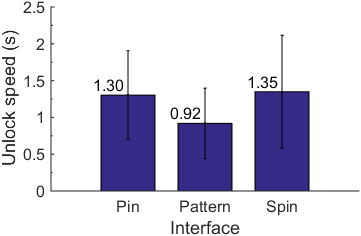
\includegraphics[width=0.7\columnwidth]{figures/analysis_1_interface_speed_bar.png}
  \caption{Average unlock time across interfaces}~\label{fig:unlock_speed_bar}
\end{figure}

\subsubsection{Differences across participants}
The average unlock times of different participants differ significantly, even averaged across all interfaces. %UPDATE: analysis_2_interface_speed_differences_between_users_anova.jpg
Thus, users were subsequently grouped into "slow" and "fast" categories using standard 2 group k-means clustering. For "fast" users, again only the pattern interface was observed to be significantly faster than the Pin and Spin interfaces. However, for "slow" users, significant differences were observed between all interface unlock speeds, with the Spin lock being slower than the Pin lock.  
 %UPDATE: analysis_2_interface_speed_slow_users_posthoc.txt

\subsubsection{Differences between password difficulties} 
Statistically significant differences were observed in the average unlock times of the various password difficulty levels, even averaged across all interfaces (Anova: $F_2=503.01$, $p < 0.001$).  %UPDATE: analysis_3_pwdcategories_speed_anova.jpg
with average unlock times increasing with password difficulty.  %UPDATE: analysis_3_pwdcategories_speed_anova_posthoc
Examining attempts from each password level independently, the results differ somewhat from those report above. These are shown in Figure ~\ref{fig:analysis_3_speed_bar}. For medium passwords, again the Pattern interface was significantly faster, with no significant difference between Spin and PIN interfaces. However, for Easy passwords, the Spin was significantly slower than the PIN. For Hard passwords, the PIN was significantly slower than the Spin.

\begin{figure}[h]
  \centering
  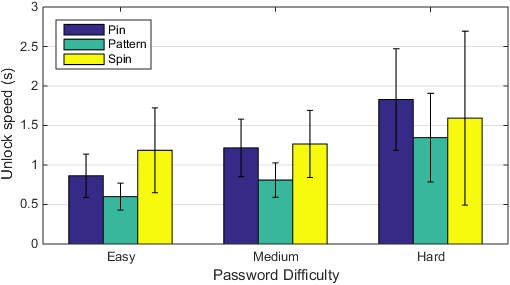
\includegraphics[width=0.9\columnwidth]{figures/analysis_3_speed_bar.png}
  \caption{Average unlock time across interfaces, across different password difficulty levels}~\label{fig:analysis_3_speed_bar}
\end{figure}  

%add bar graph!!!
%UPDATE: analysis_3_pwdcategories_speed_anova_easy.jpg
%UPDATE: analysis_3_pwdcategories_speed_anova_easy_posthoc.txt
%UPDATE: analysis_3_pwdcategories_speed_anova_hard.jpg
%UPDATE: analysis_3_pwdcategories_speed_anova_hard_posthoc.txt

\subsubsection{Differences across interface orders (counterbalancing)}
 Participants who tested the pattern interface first were, averaged across all three interfaces, significantly slowest (Anova: $F_2=33.47$, $p < 0.001$). Pattern-first participants were significantly slower than Pin-first participants on all three interfaces. They were also significantly slower than Spin-first users on all but the Pin interface.  Average speeds for the three user groups across interfaces are provided in Figure ~\ref{fig:analysis_4_speed_bar}. \\

\begin{figure}[h]
  \centering
  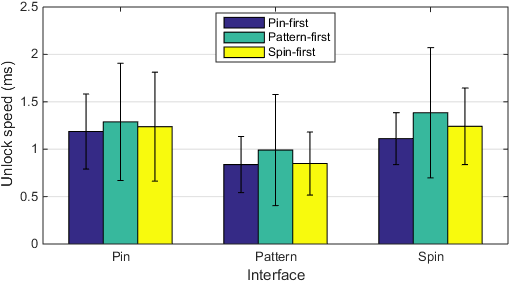
\includegraphics[width=0.85\columnwidth]{figures/analysis_4_speed_bar.png}
  \caption{Average unlock time across interfaces, across different interface-first user groups}~\label{fig:analysis_4_speed_bar}
\end{figure}


\subsubsection{Learning effect for entering new password}
Learning effect is observed in unlock speeds between the 1st, 2nd, and 3rd trials on each given password, averaged across passwords and interfaces. For each interface, statistically significant differences are observed across trials, with the 1st trial being slowest for all interfaces ($F_{2} = 28.24$, $p<0.05$). However, with learning effect minimized by only consider the 3rd trials, the average unlock speeds of all interfaces are still statistically significant ($F_{2} = 18.84$, $p<0.05$) and it aligns the the overall unlock speed results. 

\subsection{Error Rate}
Significant differences exist in error rates for each interface, averaged across all trials (Anova: $F_{2} = 19.78.84$, $p<0.01$), as shown in Figure~\ref{fig:unlock_error_rate_bar} . The Spin lock had a significantly higher error rate, validated by Tukey-Kramer post-hoc test ($p(Pin, Pattern) < 0.01 $, $p(Spin,Pattern)< 0.01$), but no significant difference was observed between Pin and Pattern locks ($p(Spin,Pattern)> 0.5$).  

 %UPDATE analysis_1_interface_error_rate_anova.jpg
%UPDATE analysis_1_interface_error_rated_anova_pin_vs_pattern.jpg 

\begin{figure}[h]
  \centering
  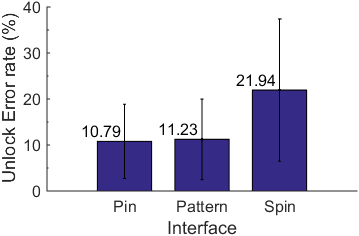
\includegraphics[width=0.7\columnwidth]{figures/analysis_1_interface_error_rate_bar.png}
  \caption{Average unlock error rate across interfaces}~\label{fig:unlock_error_rate_bar}
\end{figure}

\subsubsection{Differences across participants}
No significant differences were observed in the average unlock error rates for all interfaces across participants. Grouping participants into "error prone" and "not error prone" categories using standard 2 group k-means clustering produced similar results to those for all participants. 
 %UPDATE: analysis_2_interface_error_rate_error_prone_users_posthoc.txt
%UPDATE: analysis_2_interface_error_rate_not_error_prone_users_posthoc.txt

\subsubsection{Differences between password difficulties} 
Examining each password level independently, the results confirm those reported above: considering easy, medium and hard passwords separately, no statistical difference was observed between pin and pattern error rates, while the Spin interface was consistently more error-producing. Average error rates for each difficulty level are provided in Figure \ref{fig:unlock_error_rate_difficulty_bar}. As expected, hard passwords have a significantly higher error rate, but no significant difference was observed between medium and easy passwords, averaged across interfaces. 
%UPDATE: analysis_3_pwdcategories_error_rate_anova_easy_posthoc.txt
%UPDATE: analysis_3_pwdcategories_error_rate_anova_medium_posthoc.txt
%UPDATE: analysis_3_pwdcategories_error_rate_anova_hard_posthoc.txt
%UPDATE:analysis_3_pwdcategories_error_rate_anova_easy.jpg
%UPDATE:analysis_3_pwdcategories_error_rate_anova_medium.jpg
 %UPDATE:analysis_3_pwdcategories_error_rate_anova_hard.jpg
 %UPDATE: analysis_3_pwdcategories_error_rate_anova_hard_posthoc.txt
 %UPDATE:analysis_3_pwdcategories_error_rate_anova_hard_posthoc.txt
 \begin{figure}[h]
   \centering
   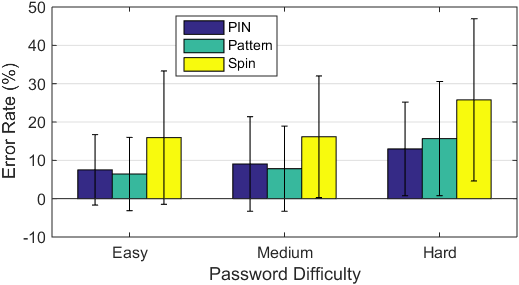
\includegraphics[width=0.9\columnwidth]{figures/analysis_3_error_bar.png}
   \caption{Average unlock error rate across interfaces}~\label{fig:unlock_error_rate_difficulty_bar}
 \end{figure}

\subsubsection{Differences across interface orders (counterbalancing)}
For participants who tested the Pattern and Spin interfaces first, the Spin lock was again observed to have a significantly higher error rate than either the Pattern or Pin interfaces. However, for users who tested the Pin first, while error rates for the Spin lock were significantly higher than for the Pin, they were not significantly higher than for the Pattern lock. 

\subsection{User Acceptance}
\begin{figure}[b]
	\centering
	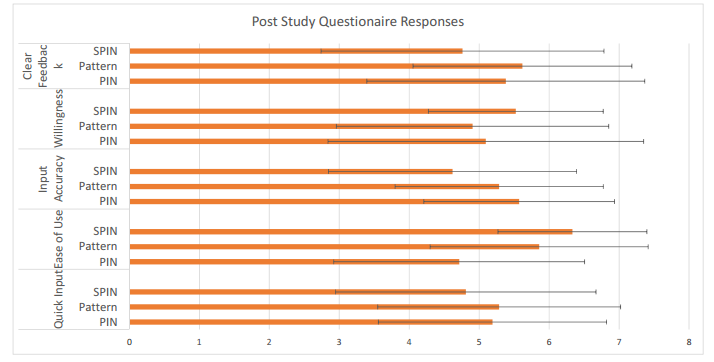
\includegraphics[width=1\columnwidth]{figures/Responses.png}
	\caption{Questionaire Responses on User Acceptance : Bar Graphs represent the average responses , Error Bars represent Standard Deviation}~\label{fig:Responses}
\end{figure}
 Figure~\ref{fig:Responses} shows the average Post-Experiment survey responses for each interface using NASA-TLX.  The Friedman Test is used to assess the participants' responses. Differences between average responses on quickness of password entry, clarity of input feedback and willingness to adopt the interface are shown to be insignificant. However, significant results have been reported for two categories: ease of use and input accuracy.

There is a significant difference in ease of use between the three interfaces ($\chi^{2} = 13.774$, df = 2, $p_{PIN,\:PATTERN, \:SPIN} = 0.001 < 0.05$).  Furthermore, the Freidman test reported significant differences for the ease of use of Spin Lock  Interfaces in comparison with PIN locking   ($p_{SPIN,\:PIN}$ using Conover's $F, df = 1 >  0.450$) \comment{in which direction? which is better?}.  Moreover, Pattern Lock Interfaces were found to be significantly easier to use than PIN interfaces among all password complexities \comment{confused. do you mean like you tested each difficulty level seaprately?} ($p_{Pattern,\:PIN} > 0.450$). 

Regarding input accuracy, there is a significant difference between the three interfaces ($\chi^{2} = 5.792$, df = 2, $p_{PIN,\:PATTERN, \:SPIN} < 0.01$, df = 2). A post-hoc multiple comparisons test identified significant differences for the input accuracy of the Pin lock in comparison with the Spin lock \comment{again, which is higher?!} ($p_{PIN,\:SPIN}$ using Conover's $F, df = 1 >  0.449$).  Users have also reported, in the free-form feedback section, that accurate password entry is much easier using the PIN lock than the Spin interface.

\section{Discussion}
% H1 The spin lock and pattern lock will have similar unlock times that are significantly higher than the PIN lock, given same password complexity.
% H2 The spin lock and pattern lock will have significantly higher error rates as compared to the PIN lock.
% H3 The spin lock will have a lower user acceptance rate than the PIN and pattern locks.
The results presented above run counter to our hypotheses, regarding unlock speed, error rate, and user acceptance. A summary of these results is presented in Table  and further ~\ref{tab:hypothesis_result} discussed below. In short, the newly designed Spin lock could not could not surpass the performance of both the existing PIN and pattern locks on Android in terms of speed or error rate. However, speed and error rates are not incomparable and users enjoy interacting with the spin lock more than the existing PIN and pattern locks, being surprisingly well received by the test participants.

\begin{table}[h]
\centering
\small
  \begin{tabularx}{\columnwidth}{c  X  X}
    \toprule
     & \multicolumn{1}{c}{\small\textit{ Predicted}}  & \multicolumn{1}{c}{\small\textit{ Result}}\\
    \midrule
    \small\textbf{H1} & Spin lock and pattern lock have similar unlock speed  \newline
    								      Spin lock and pattern lock are slower than PIN lock  & 				  
    								      Spin lock and PIN lock have similar unlock speed \newline
    								      Pattern lock is fast than spin lock and PIN lock \\
    \midrule
    \small\textbf{H2} & Higher error rates: spin and pattern lock  \newline
    								      Lowest error rate: PIN lock & 
				 						Highest error rate: spin lock\newline
    								      Lower and similar error rates: PIN and pattern lock\\    \midrule
    \small\textbf{H3} &Spin lock have lowest acceptance  
    			       & Spin lock have highest acceptance\\ 
    \bottomrule
  \end{tabularx}
  \caption{Hypothesis and results}~\label{tab:hypothesis_result}
\end{table}

\subsubsection{Unlock Speed}\label{sec:discussion_unlock_speed}

The Pattern lock had, on average, a significantly faster unlock time than the Pin (and also Spin) locks. This contradicts the results from ~\cite{von_zezschwitz_patterns_2013}, which reports an average Pin unlock time of 1.501 s and Pattern unlock time of 3.136 s. This Pattern unlock time is over twice as slow as the average times we observed for both Hard Pattern passwords ad for Slow Users, while the Pin time is approximately twice as slow as for Easy passwords, but similar to those of Hard passwords and slow users. This disparity is likely due to differences in the complexity of tested passwords in the two studies.  ~\cite{von_zezschwitz_patterns_2013} used only one level of difficulty, with all PIN passwords consisting of four digits and all pattern passwords being five-stroke patterns on a 3x3 grid, which were directly compared. However, our finger-movement based password comparison would results in a four digit Pin being categorized as an easy password, while a five-stroke Pattern would be categorized as hard. Given that the average unlock times \textit{across all interfaces} increased with password complexity in our study, we believe that our results regarding Pattern and Pin speeds are more representative of the actual unlock speeds of the interfaces. 

Another possible reason for the disparity is the inclusion of an ``undo'' button in the Pin lock in ~\cite{von_zezschwitz_patterns_2013}'s design. Thus, users were able to "fix" mistakes in a PIN unlock trial, but not in a Pattern trial. Our design, however, did not provide undo options for any of the interfaces. However, we also did not include unsuccessful attempts in the calculations of unlock speed. Thus, one might expect higher Pin unlock times in ~\cite{von_zezschwitz_patterns_2013}'s study, since "undo"s might lengthen trial time, yet this is not the case. Yet, the lack of an undo button may have caused some confusion since it is incorporated in the stock Android Pin lock; one user commented that they required the back-space button. 

While the pattern lock was also significantly faster than the spin lock, the Pin lock was \textit{not} significantly faster. This is surprising given that the Spin lock is a new interface for all users (whereas many have used the Pin and Pattern interfaces in the past), and would be expected to increase unlock times. Multiple users acknowledged this need for \comment{adjustment as in practice?}adjustment to the Spin interface, but also that it was the "fastest [and] most enjoyable" after they began to master it. The above suggest that the Spin interface speeds could surpass the traditional PIN and perhaps approach the Pattern speeds given further practice. 

Furthermore, while for Hard and Easy passwords a significant difference was observed between Spin and Pin passwords, this was not the case for Medium passwords. Given that users were presented Easy trials first, they might not have yet adjusted to the interface, and thus the disparity may only exist between Pin and Spin for Easy passwords due to learning effects. 
% Learning effects: the fast users for spin and pin performs on the same level, while slow users for pin lock are slower indicates 1), not all users have learned the interface. 2), once learned, spin lock has performance as good as pin lock - confirms with the overall result



% Learning effect also happens for each new password given. After removing the attempts where the user is still trying to learn the password, the result confirms with the overall result.



% Strangely, interface order seem to have significant effect on user's performance. Users start with pattern seem to have slightly slower performance. A possible explanation is the users ``let their guard down'' when they start the test with the presumably easiest interface. However, as the trails are randomized, this should have negligible effect on the overall result.


\subsubsection{Error Rate}

Again, contrary to the results in ~\cite{von_zezschwitz_patterns_2013}, where Pin was observed to have a significantly slower error rate (5\%) than Pattern (16\%), we observed no significant difference in error rates of the two (\texttildelow11\%), regardless of password difficulty, or users being "error-prone" or not "error-prone". As mentioned in ~\ref{sec:discussion_unlock_speed}, this may be again due complexity of passwords tested in our study and our attempt to make them comparable across interfaces. 

We found the spin lock to have a statistically higher error rate of 21.9\% which was nearly double the error rate of the PIN and pattern locks, and was in line with our hypothesis that it would be higher than the PIN lock. However, we cannot discount the possibility that this is due to the novelty of the interface for participants. Although participants were given 5 minutes to practice beforehand, most users did not use the entire time which may have been insufficient to familiarize themselves with the interface. Future experiments could be improved by enforcing longer practice sessions and a ''test" to ensure competence. 

Our hypothesis that the Pattern and Spin locks would have similar error rates was also disproved. Yet, unlike ~\cite{von_zezschwitz_patterns_2013}, the gesture-based Pattern lock did not have significantly higher error rates than the Pin interface. This may suggest that gesture-based input does not lead to higher error-rates, and that the higher errors for the Spin interface are a result of unfamiliarity, which would be expected to decline with practice. 


\subsubsection{User Acceptance}
% although quantitative data shows spin sucks, users dont feel the same way
% they are indifferent to input speed, feedback and willingness to adopt

% they did feel error rate is lower with PIN, which aligned with quantitative result 

% but they feel spin is more usable, despite of it's a novel interface
% people's comment highlighted that the lack of practice maybe the reason for lower accuracy and willingness to adopt. 
Although the quantitative data on unlock speed and error rate indicated that participants generally perform better with pattern or PIN locks, our survey results showed that performance does not translate well into user acceptance. In the post study survey, participants are indifferent to the three interfaces in terms of input speed, input feedback and willingness to adopt the interface. However, users did feel that inputting with PIN lock is more accurate than the spin lock, which aligned with quantitative error rate results. Interestingly, despite the quantitative error rate of spin lock being almost twice as high compared to pattern lock, participants felt these two lock screens have similar unlock accuracy. This could be due to users perceiving gesture based interactions in the same way. Most surprisingly, user also rated spin lock to be most usable among all 3 interfaces. Although participants also indicated spin lock does not have the best accuracy, they still liked the interface and enjoyed interacting with it. Some users also reported that if more practice were given, they would have performed better with the spin lock. The lack of practice on the new interface might be the reason for users' indifference toward adopting the new spin interface despite of it being rated as highly usable. 

\comment{this shouldn't be in here.. should be in speed or error rate discussion}
However, based on the participant acquisition questionnaires, 47.62\% of the participants used the pattern lock screen regularly compared to the 23.81\% that used PIN locks. As a result, this might explain why the pattern lock turned out to have the highest unlock speed, lowest error rate, and high user acceptance among the participants. 

\subsection{Conclusion}
% usability-wise, spin lock is slower and more error-prone, but it matches up well
% in fact, users receives this interface well
% Learning effect might be the reason error rate is higher
% Had to sacrifice usability for additional security - good thing is the users are ok with it!
In this study, we designed a new lock screen interface inspired by the physical combinational lock, and compared it to the existing Android PIN and pattern locks. Since this new interface requires complex and novel interactions, it was no surprise that it produced \comment{not longer though.. maybe ``not surpass the industry standards''?}longer unlock times and higher error rates. The high error rates may be a result of unusual circular gestures to spin the virtual dial, which are less common than straight-line strokes and swipes. With further exposure to the interface, error rates would likely improve. However, even with such little exposure, the Spin interface had comparable unlock speeds to the standard Pin lock. Furthermore, survey results suggest that participants actually find the Spin and Pattern locks easier to user than the Pin lock. This may be due to the interesting and intuitive interactions of the Spin and Pattern locks. 

Due to the scope of the study, our participant pools was limited to university students and the results may not generalize well to other populations. Furthermore, due to the availability of our participants, each trial is limited to 15 to 20 minutes, and some participants could not adjust to the new interface over a the period of time: their first exposure to it was during the experiment, with only 5 minutes of practice time. 

Another limitation of this research is the selection of tested passwords. There is little existing literature on creating comparable passwords across different interfaces, which is necessary to compare their usability. Further research is required to validate our method of determining password complexity. Furthermore, the selected passwords may not be representative of passwords that will be actually selected by users. Further studies are required into the performance, and security, of the Spin interface for user-selected passwords, as compared to the Pin and Pattern interfaces, given the differences in unlock speeds across different password complexities. Other research directions include utilizing Fitts's law as a measure of human performance, and also studying the security aspect of the Spin lock with respect to shoulder surfing  and smudge attacks

\comment{do we not mention the security benefit here at all?}
Overall, we were able to demonstrate that the alternative spin lock created in this study achieves great user acceptance, despite having more more complicated interactions. We expect the spin lock to deliver same or higher performance compared to the pin lock in real-world use, where the user will have fully acclimatized to the interface. Further work on the Spin lock could provide improvements in lock-screen security and user experience, which could be easily passed on to mobile device users. 

%%%
%%% CHI Paper Specs
%%%
\iffalse
\section{Page Size and Columns}
On each page your material should fit within a rectangle of 7 $\times$
9.25 inches (18 $\times$ 23.5 cm), centered on a US Letter page (8.5
$\times$ 11 inches), beginning 0.75 inches (1.9 cm) from the top of
the page, with a 0.33 inches (0.85 cm) space between two 3.3 inches
(8.4 cm) columns. Right margins should be justified, not
ragged. Please be sure your document and PDF are US letter and not A4.


\section{Typeset Text}
The styles contained in this document have been modified from the
default styles to reflect ACM formatting conventions. For example,
content paragraphs like this one are formatted using the Normal style.


\LaTeX\ sometimes will create overfull lines that extend into columns.
To attempt to combat this, the \texttt{.cls} file has a command,
\texttt{{\textbackslash}sloppy}, that essentially asks \LaTeX\ to
prefer underfull lines with extra whitespace.  For more details on
this, and info on how to control it more finely, check out
{\url{http://www.economics.utoronto.ca/osborne/latex/PMAKEUP.HTM}}.

\subsection{Title and Authors}

Your paper's title, authors and affiliations should run across the
full width of the page in a single column 17.8 cm (7 in.) wide.  The
title should be in Helvetica or Arial 18-point bold.  Authors' names
should be in Times New Roman or Times Roman 12-point bold, and
affiliations in 12-point regular.  

See \texttt{{\textbackslash}author} section of this template for
instructions on how to format the authors. For more than three
authors, you may have to place some address information in a footnote,
or in a named section at the end of your paper. Leave one 10-point
line of white space below the last line of affiliations.

\subsection{Abstract and Keywords}

Every submission should begin with an abstract of about 150 words,
followed by a set of Author Keywords and ACM Classification
Keywords. The abstract and keywords should be placed in the left
column of the first page under the left half of the title. The
abstract should be a concise statement of the problem, approach, and
conclusions of the work described. It should clearly state the paper's
contribution to the field of HCI\@.

\subsection{Normal or Body Text}

Please use a 10-point Times New Roman or Times Roman font or, if this
is unavailable, another proportional font with serifs, as close as
possible in appearance to Times Roman 10-point. Other than Helvetica
or Arial headings, please use sans-serif or non-proportional fonts
only for special purposes, such as source code text.

\subsection{First Page Copyright Notice}
This template include a sample ACM copyright notice at the bottom of
page 1, column 1.  Upon acceptance, you will be provided with the
appropriate copyright statement and unique DOI string for publication.
Accepted papers will be distributed in the conference
publications. They will also be placed in the ACM Digital Library,
where they will remain accessible to thousands of researchers and
practitioners worldwide. See
\url{http://acm.org/publications/policies/copyright_policy} for the
ACM’s copyright and permissions policy.

%%%

\subsection{Subsequent Pages}

On pages beyond the first, start at the top of the page and continue
in double-column format.  The two columns on the last page should be
of equal length.

\begin{figure}
\centering
  
\includegraphics[width=0.9\columnwidth]{figures/sigchi-logo}
  \caption{Insert a caption below each figure. Do not alter the
    Caption style.}~\label{fig:figure1}
\end{figure}

\subsection{References and Citations}

Use a numbered list of references at the end of the article, ordered
alphabetically by last name of first author, and referenced by numbers
in 
brackets~\cite{acm_categories,ethics,Klemmer:2002:WSC:503376.503378}.
Your references should be published materials accessible to the
public. Internal technical reports may be cited only if they are
easily accessible (i.e., you provide the address for obtaining the
report within your citation) and may be obtained by any reader for a
nominal fee. Proprietary information may not be cited. Private
communications should be acknowledged in the main text, not referenced
(e.g., ``[Borriello, personal communication]'').

References should be in ACM citation format:
\url{http://acm.org/publications/submissions/latex_style}. This
includes citations to internet
resources~\cite{acm_categories,cavender:writing,CHINOSAUR:venue,psy:gangnam}
according to ACM format, although it is often appropriate to include
URLs directly in the text, as above.


% Use a numbered list of references at the end of the article, ordered
% alphabetically by first author, and referenced by numbers in
% brackets~\cite{ethics, Klemmer:2002:WSC:503376.503378,
%   Mather:2000:MUT, Zellweger:2001:FAO:504216.504224}. For papers from
% conference proceedings, include the title of the paper and an
% abbreviated name of the conference (e.g., for Interact 2003
% proceedings, use \textit{Proc. Interact 2003}). Do not include the
% location of the conference or the exact date; do include the page
% numbers if available. See the examples of citations at the end of this
% document. Within this template file, use the \texttt{References} style
% for the text of your citation.

% Your references should be published materials accessible to the
% public.  Internal technical reports may be cited only if they are
% easily accessible (i.e., you provide the address for obtaining the
% report within your citation) and may be obtained by any reader for a
% nominal fee.  Proprietary information may not be cited. Private
% communications should be acknowledged in the main text, not referenced
% (e.g., ``[Robertson, personal communication]'').

\begin{table}
  \centering
  \begin{tabular}{r c c}
    \toprule
    & \multicolumn{2}{c}{\small{\textbf{Caption}}} \\
    \cmidrule(r){2-3}
    {\small\textbf{Objects}}
    & {\small \textit{Pre-2002}}
    & {\small \textit{Current}} \\
    \midrule
    Tables & Above & Below \\
    Figures & Below & Below \\
    \bottomrule
  \end{tabular}
  \caption{Table captions should be placed below the table. We
    recommend table lines be 1 point, 25\% black. Minimize use of
    unnecessary table lines.}~\label{tab:table1}
\end{table}

\section{Sections}

The heading of a section should be in Helvetica or Arial 9-point bold,
all in capitals. Sections should \textit{not} be numbered.

\subsection{Subsections}

Headings of subsections should be in Helvetica or Arial 9-point bold
with initial letters capitalized.  For sub-sections and
sub-subsections, a word like \emph{the} or \emph{of} is not
capitalized unless it is the first word of the heading.

\subsubsection{Sub-subsections}

Headings for sub-subsections should be in Helvetica or Arial 9-point
italic with initial letters capitalized.  Standard
\texttt{{\textbackslash}section}, \texttt{{\textbackslash}subsection},
and \texttt{{\textbackslash}subsubsection} commands will work fine in
this template.

\section{Figures/Captions}

Place figures and tables at the top or bottom of the appropriate
column or columns, on the same page as the relevant text (see
Figure~\ref{fig:figure1}). A figure or table may extend across both
columns to a maximum width of 17.78 cm (7 in.).

\begin{figure*}
  \centering
  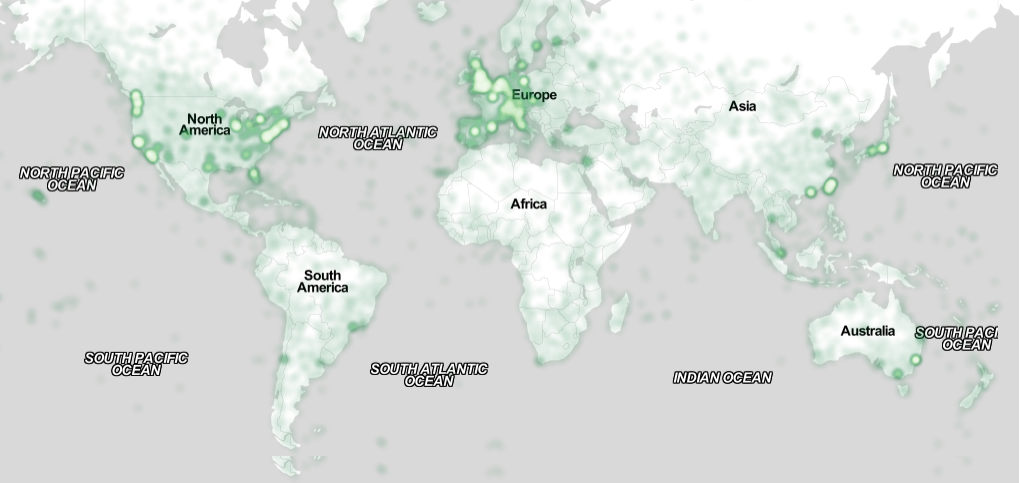
\includegraphics[width=2\columnwidth]{figures/map}
  \caption{In this image, the map maximizes use of space. You can make
    figures as wide as you need, up to a maximum of the full width of
    both columns. Note that \LaTeX\ tends to render large figures on a
    dedicated page. Image: \ccbynd~ayman on
    Flickr.}~\label{fig:figure2}
\end{figure*}

Captions should be Times New Roman or Times Roman 9-point bold.  They
should be numbered (e.g., ``Table~\ref{tab:table1}'' or
``Figure~\ref{fig:figure1}''), centered and placed beneath the figure
or table.  Please note that the words ``Figure'' and ``Table'' should
be spelled out (e.g., ``Figure'' rather than ``Fig.'') wherever they
occur. Figures, like Figure~\ref{fig:figure2}, may span columns and
all figures should also include alt text for improved accessibility.
Papers and notes may use color figures, which are included in the page
limit; the figures must be usable when printed in black-and-white in
the proceedings.

The paper may be accompanied by a short video figure up to five
minutes in length. However, the paper should stand on its own without
the video figure, as the video may not be available to everyone who
reads the paper.  

\subsection{Inserting Images}
When possible, include a vector formatted graphic (i.e. PDF or EPS).
When including bitmaps,  use an image editing tool to resize the image
at the appropriate printing resolution (usually 300 dpi).

\section{Language, Style and Content}

The written and spoken language of SIGCHI is English. Spelling and
punctuation may use any dialect of English (e.g., British, Canadian,
US, etc.) provided this is done consis- tently. Hyphenation is
optional. To ensure suitability for an international audience, please
pay attention to the following:

\begin{itemize}
\item Write in a straightforward style.
\item Try to avoid long or complex sentence structures.
\item Briefly define or explain all technical terms that may be
  unfamiliar to readers.
\item Explain all acronyms the first time they are used in your
  text---e.g., ``Digital Signal Processing (DSP)''.
\item Explain local references (e.g., not everyone knows all city
  names in a particular country).
\item Explain ``insider'' comments. Ensure that your whole audience
  understands any reference whose meaning you do not describe (e.g.,
  do not assume that everyone has used a Macintosh or a particular
  application).
\item Explain colloquial language and puns. Understanding phrases like
  ``red herring'' may require a local knowledge of English.  Humor and
  irony are difficult to translate.
\item Use unambiguous forms for culturally localized concepts, such as
  times, dates, currencies, and numbers (e.g., ``1--5--97'' or
  ``5/1/97'' may mean 5 January or 1 May, and ``seven o'clock'' may
  mean 7:00 am or 19:00). For currencies, indicate equivalences:
  ``Participants were paid {\fontfamily{txr}\selectfont \textwon}
  25,000, or roughly US \$22.''
\item Be careful with the use of gender-specific pronouns (he, she)
  and other gendered words (chairman, manpower, man-months). Use
  inclusive language that is gender-neutral (e.g., she or he, they,
  s/he, chair, staff, staff-hours, person-years). See the
  \textit{Guidelines for Bias-Free Writing} for further advice and
  examples regarding gender and other personal
  attributes~\cite{Schwartz:1995:GBF}. Be particularly aware of
  considerations around writing about people with disabilities.
\item If possible, use the full (extended) alphabetic character set
  for names of persons, institutions, and places (e.g.,
  Gr{\o}nb{\ae}k, Lafreni\'ere, S\'anchez, Nguy\~{\^{e}}n,
  Universit{\"a}t, Wei{\ss}enbach, Z{\"u}llighoven, \r{A}rhus, etc.).
  These characters are already included in most versions and variants
  of Times, Helvetica, and Arial fonts.
\end{itemize}

\section{Accessibility}
The Executive Council of SIGCHI has committed to making SIGCHI
conferences more inclusive for researchers, practitioners, and
educators with disabilities. As a part of this goal, the all authors
are asked to work on improving the accessibility of their
submissions. Specifically, we encourage authors to carry out the
following five steps:
\begin{enumerate}
\item Add alternative text to all figures
\item Mark table headings
\item Add tags to the PDF
\item Verify the default language
\item Set the tab order to ``Use Document Structure''
\end{enumerate}
For more information and links to instructions and resources, please
see: \url{http://chi2016.acm.org/accessibility}.  The
\texttt{{\textbackslash}hyperref} package allows you to create well tagged PDF files,
please see the preamble of this template for an example.

\section{Page Numbering, Headers and Footers}
Your final submission should not contain footer or header information
at the top or bottom of each page. Specifically, your final submission
should not include page numbers. Initial submissions may include page
numbers, but these must be removed for camera-ready. Page numbers will
be added to the PDF when the proceedings are assembled.

\section{Producing and Testing PDF Files}

We recommend that you produce a PDF version of your submission well
before the final deadline.  Your PDF file must be ACM DL
Compliant. The requirements for an ACM Compliant PDF are available at:
{\url{http://www.sheridanprinting.com/typedept/ACM-distilling-settings.htm}}.

Test your PDF file by viewing or printing it with the same software we
will use when we receive it, Adobe Acrobat Reader Version 10. This is
widely available at no cost. Note that most
reviewers will use a North American/European version of Acrobat
reader, so please check your PDF accordingly.

When creating your PDF from Word, ensure that you generate a tagged
PDF from improved accessibility. This can be done by using the Adobe
PDF add-in, also called PDFMaker. Select Acrobat | Preferences from
the ribbon and ensure that ``Enable Accessibility and Reflow with
tagged Adobe PDF'' is selected. You can then generate a tagged PDF by
selecting ``Create PDF'' from the Acrobat ribbon.

\section{Conclusion}

It is important that you write for the SIGCHI audience. Please read
previous years’ proceedings to understand the writing style and
conventions that successful authors have used. It is particularly
important that you state clearly what you have done, not merely what
you plan to do, and explain how your work is different from previously
published work, i.e., the unique contribution that your work makes to
the field. Please consider what the reader will learn from your
submission, and how they will find your work useful. If you write with
these questions in mind, your work is more likely to be successful,
both in being accepted into the conference, and in influencing the
work of our field.

\section{Acknowledgments}

Sample text: We thank all the volunteers, and all publications support
and staff, who wrote and provided helpful comments on previous
versions of this document. Authors 1, 2, and 3 gratefully acknowledge
the grant from NSF (\#1234--2012--ABC). \textit{This whole paragraph is
  just an example.}

% Balancing columns in a ref list is a bit of a pain because you
% either use a hack like flushend or balance, or manually insert
% a column break.  http://www.tex.ac.uk/cgi-bin/texfaq2html?label=balance
% multicols doesn't work because we're already in two-column mode,
% and flushend isn't awesome, so I choose balance.  See this
% for more info: http://cs.brown.edu/system/software/latex/doc/balance.pdf
%
% Note that in a perfect world balance wants to be in the first
% column of the last page.
%
% If balance doesn't work for you, you can remove that and
% hard-code a column break into the bbl file right before you
% submit:
%
% http://stackoverflow.com/questions/2149854/how-to-manually-equalize-columns-
% in-an-ieee-paper-if-using-bibtex
%
% Or, just remove \balance and give up on balancing the last page.
%
\balance{}

\section{References Format}
Your references should be published materials accessible to the
public. Internal technical reports may be cited only if they are
easily accessible (i.e., you provide the address for obtaining the
report within your citation) and may be obtained by any reader for a
nominal fee. Proprietary information may not be cited. Private
communications should be acknowledged in the main text, not referenced
(e.g., ``[Golovchinsky, personal communication]'').

Use a numbered list of references at the end of the article, ordered
alphabetically by first author, and referenced by numbers in
brackets~\cite{ethics,Klemmer:2002:WSC:503376.503378}. For papers from
conference proceedings, include the title of the paper and an
abbreviated name of the conference (e.g., for Interact 2003
proceedings, use Proc.\ Interact 2003). Do not include the location of
the conference or the exact date; do include the page numbers if
available. See the examples of citations at the end of this document
and in the accompanying \texttt{BibTeX} document.

References \textit{must be the same font size as other body
  text}. References should be in alphabetical order by last name of
first author. Example reference formatting for individual journal
articles~\cite{ethics}, articles in conference
proceedings~\cite{Klemmer:2002:WSC:503376.503378},
books~\cite{Schwartz:1995:GBF}, theses~\cite{sutherland:sketchpad},
book chapters~\cite{winner:politics}, a journal issue~\cite{kaye:puc},
websites~\cite{acm_categories,cavender:writing},
tweets~\cite{CHINOSAUR:venue}, patents~\cite{heilig:sensorama}, and
online videos~\cite{psy:gangnam} is given here. This formatting is a
slightly abbreviated version of the format automatically generated by
the ACM Digital Library (\url{http://dl.acm.org}) as ``ACM Ref''. More
details of reference formatting are available at:
\url{http://www.acm.org/publications/submissions/latex_style}.

\fi

% REFERENCES FORMAT
% References must be the same font size as other body text.
\bibliographystyle{SIGCHI-Reference-Format}
\bibliography{sample}

\end{document}

%%% Local Variables:
%%% mode: latex
%%% TeX-master: t
%%% End:
